\section{Comparison Result}
\subsection{Comparison Result Between Regular Mesh and Toroidal With Same Processors Number}
Considering a regular mesh \Fig{5t5}, the best position for data injection is $P_{12}$.   Other positions, for example $P_{8}$, $P_{13}$, they don't have the same speedup efficiency.   Yet, for a toroidal $5*5$ regular mesh, each position's efficiency is equal.  \Fig{sacom5t5ci} explores the comparison result between the toroidal and corner scenario difference. 

\subsection{Comparison Result With Corner Processor and Inner Grid Processor}
For a $5*5$ regular network, the inner grid position is $P_{12}$ and the corner data injection position is $P_{0}$.  
The comparing result is \Fig{sacom5t5ci}.  

\begin{figure}[!ht]
\centering
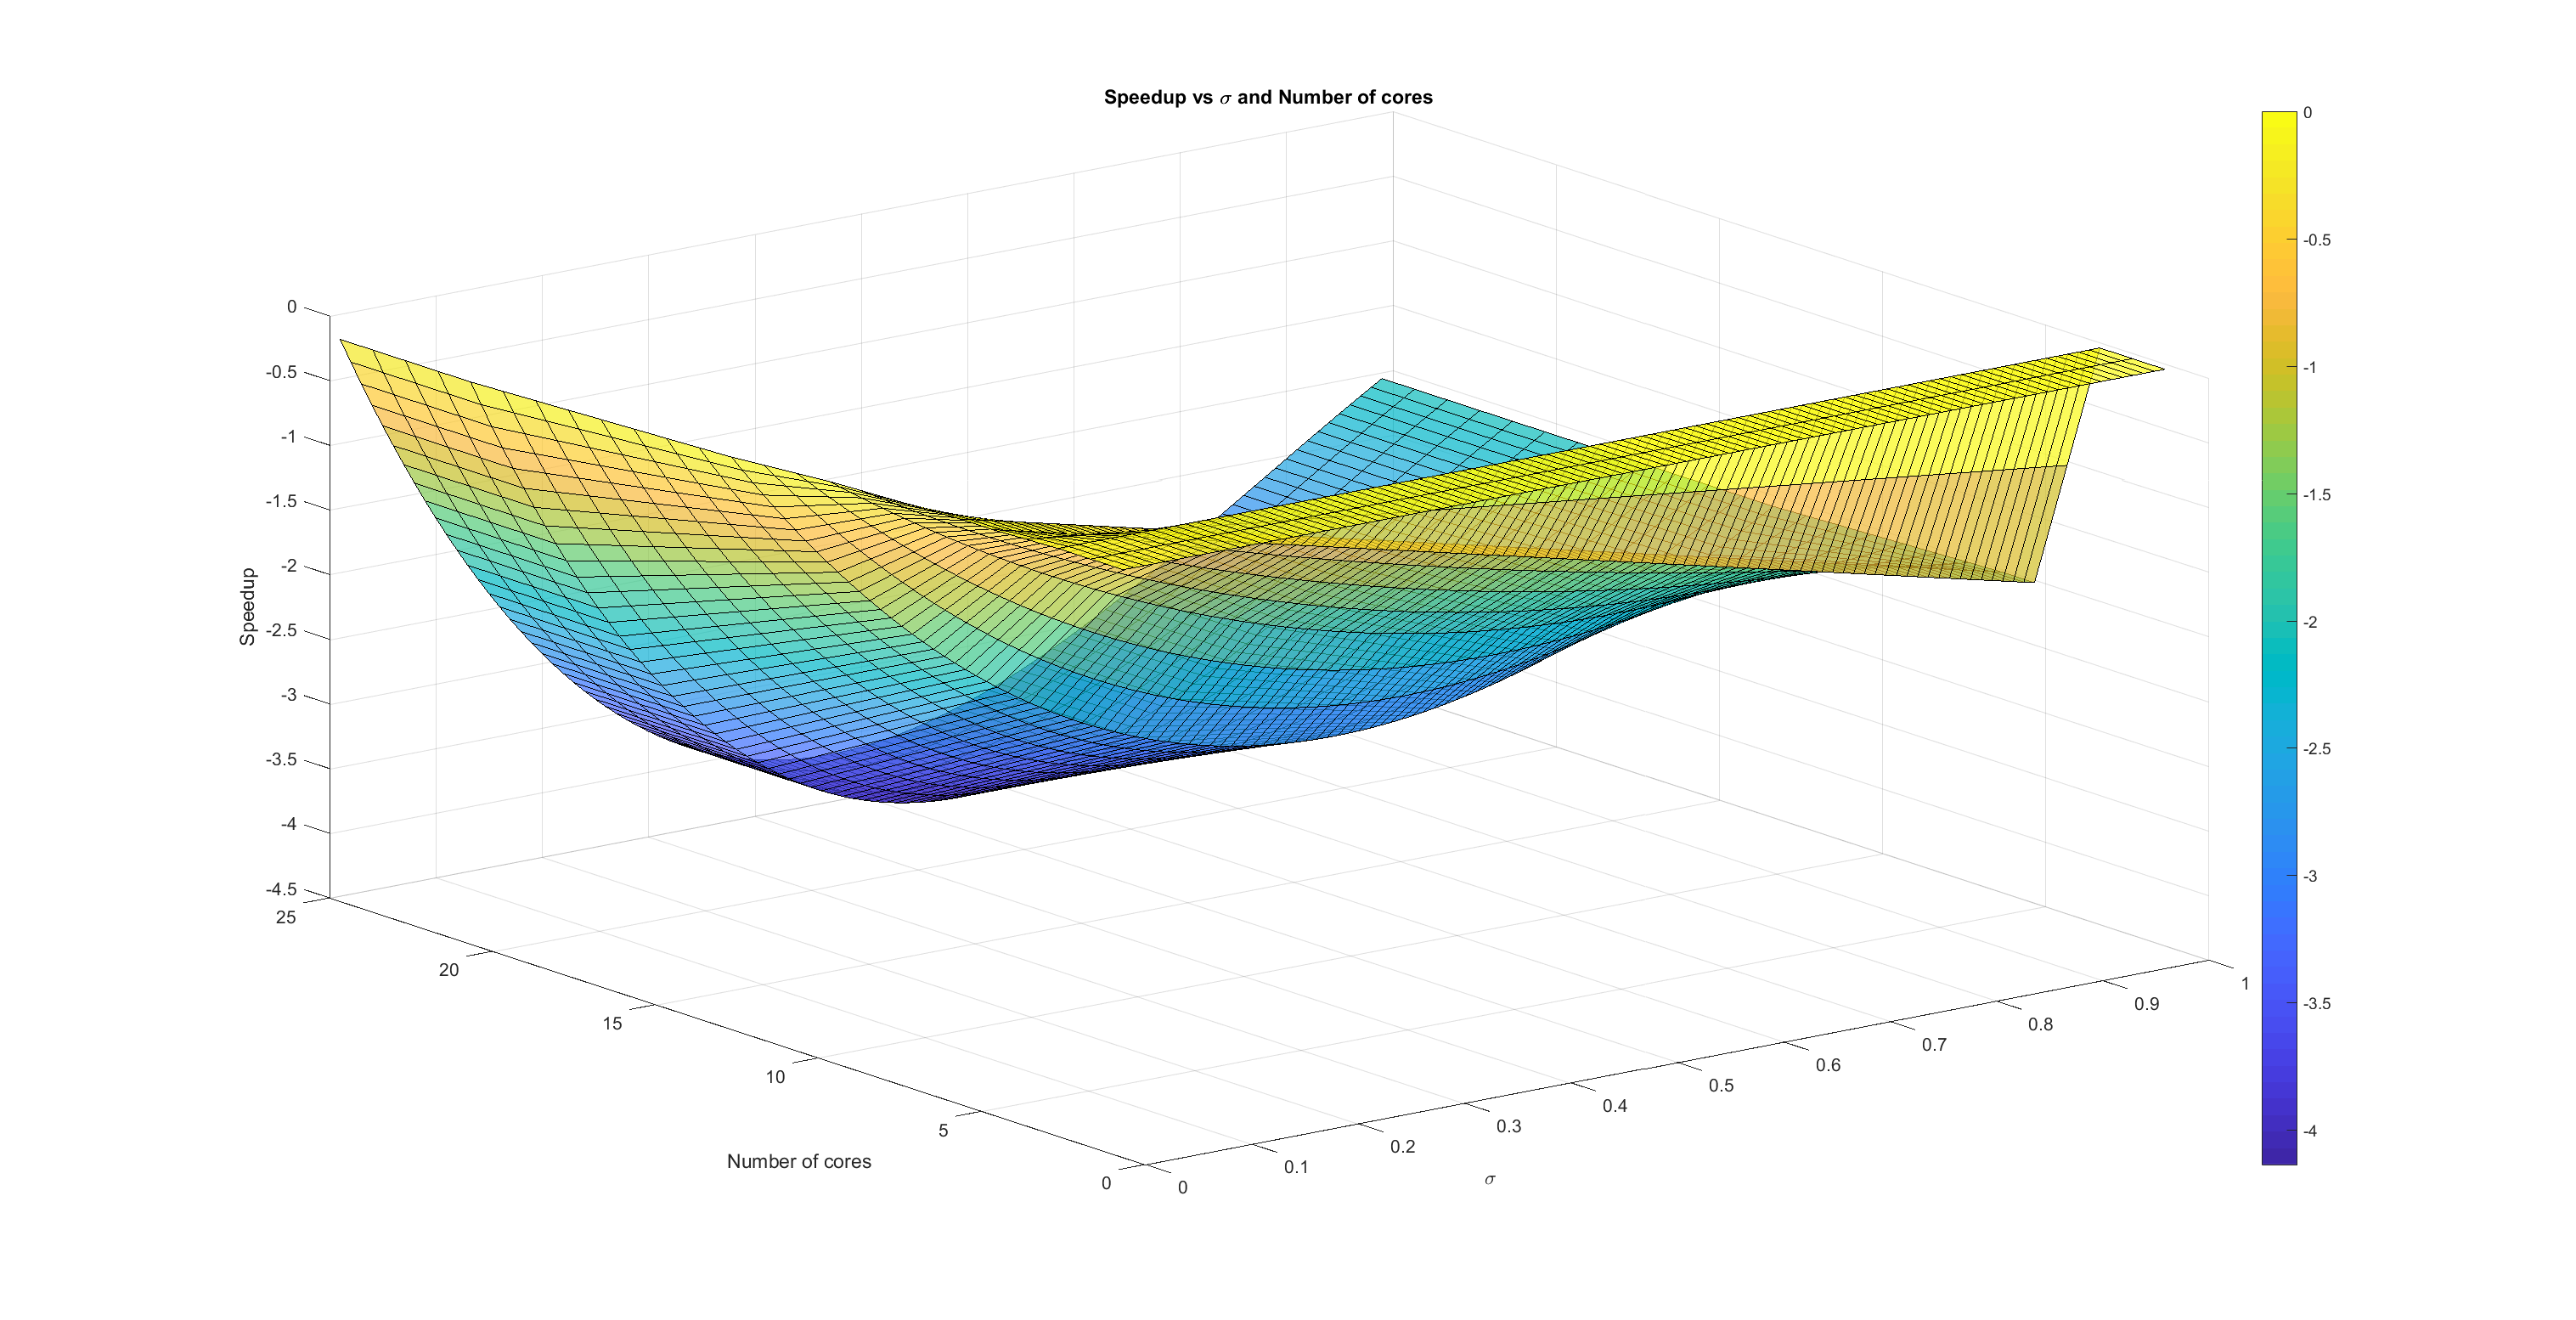
\includegraphics[width=1\columnwidth]{figure/sacom5t5ci.eps}
\caption{ Speedup difference between corner injection and inner grid injection}
\label{fig:sacom5t5ci}
\end{figure}

Generally speaking, \Fig{sacom5t5ci} says the inner grid position scenario has better performance than the corner injection option.   If the grid node is $25$ and $\sigma = 0.5$, the speedup difference is largest, which is $4$.  
\newpage

\subsection{Comparison Result Between Front-end Processor and Without Front-end Processor}

In the legend of figures,  we use 
\begin{itemize}
\item $F$ presents the processors are with front-end situation.
\item $NF$ presents the processors are without front-end situation.
\item $F\alpha_{0}$ means the $\alpha_{0}$ data fraction deployed to $P_{0}$, if the processor has front-end.
\item $NF\alpha_{0}$ means the $\alpha_{0}$ data fraction deployed to $P_{0}$, if the processor is without front-end setting.
\end{itemize}

\subsubsection{Data Injection On the Corner Processor}

\begin{figure}[!ht]
\centering
\includegraphics[width=1\columnwidth]{figure/2t2_c.eps}
\caption{The comparing result between front-end processor with without front-end processor in 2*2 regular network }
\label{fig:2t2_c}
\end{figure}

\Fig{2t2_c} says that $P_{0}$ takes more assigned task in without front-end scenario than front-end processor situation.  As the value $\sigma$ value goes up, the fractions are deployed to the deeper layers decreases.  In the limit condition, for example, $\sigma  = 1$,  there is no data transmitted to $P_{3}$ in the front-end assumption,  yet in the without front-end situation,  there is still about $10\%$ data fraction are communicated to $P_{3}$.  
\newpage

\begin{figure}[!ht]
\centering
\includegraphics[width=1\columnwidth]{figure/2t3_c.eps}
\caption{The comparing result between front-end processor with without front-end processor in 2*3 regular network }
\label{fig:2t3_c}
\end{figure}
\newpage

\Fig{2t3_c} says that $P_{0}$ takes more assigned task in without front-end scenario than front-end processor situation.  As the $\sigma$ value goes up, the fractions are deployed to the deeper levels degrades.  In the limit condition, for example, $\sigma  = 1$,  there is no data transmitted to $level_{3}$, that is, $P_{5}$ in the front-end assumption.  Yet in the without front-end situation,  there is still about $5\%$ data fraction is communicated to $P_{5}$.  
\newpage 

\begin{figure}[!ht]
\centering
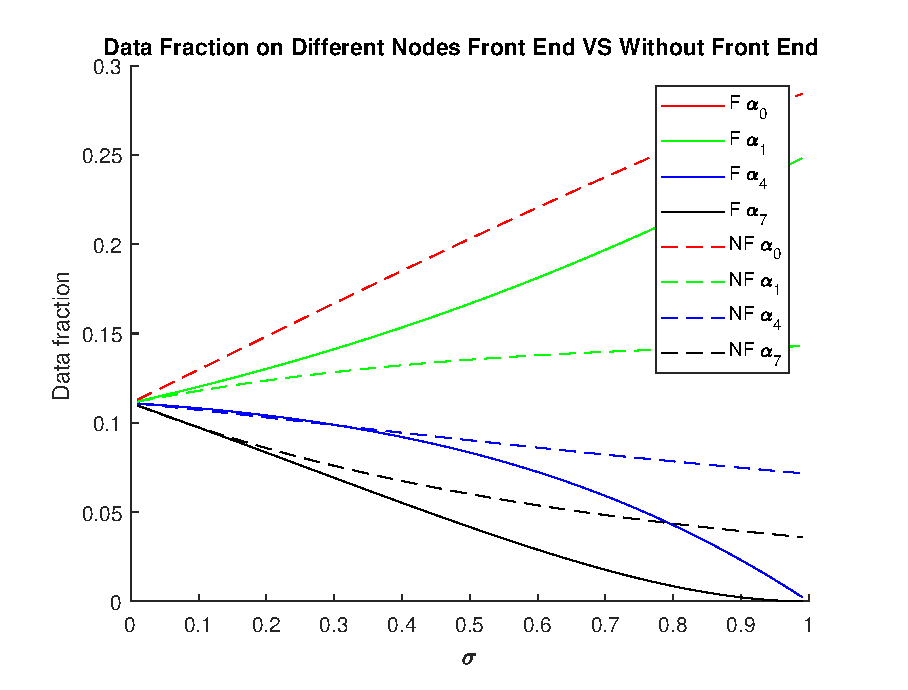
\includegraphics[width=1\columnwidth]{figure/3t3b_c.eps}
\caption{The comparing result between front-end processor with without front-end processor in 3*3 regular network injection on boundary processor }
\label{fig:3t3b_c}
\end{figure}

\Fig{3t3b_c} says that $P_{0}$ takes more assigned task in without front-end scenario than front-end processor situation.  As the $\sigma$ value goes up, the fractions are deployed to the deeper levels decreases.  In the limit condition, for example, $\sigma  = 1$,  there is no data transmitted to $level_{3}$, that is, $P_{7}$ and $P_{8}$ in the front-end assumption.  Yet in the without front-end situation,  there is still about $5\%$ data fraction is communicated to $P_{7}$ and $P_{8}$.  

\newpage 
\begin{figure}[!ht]
\centering
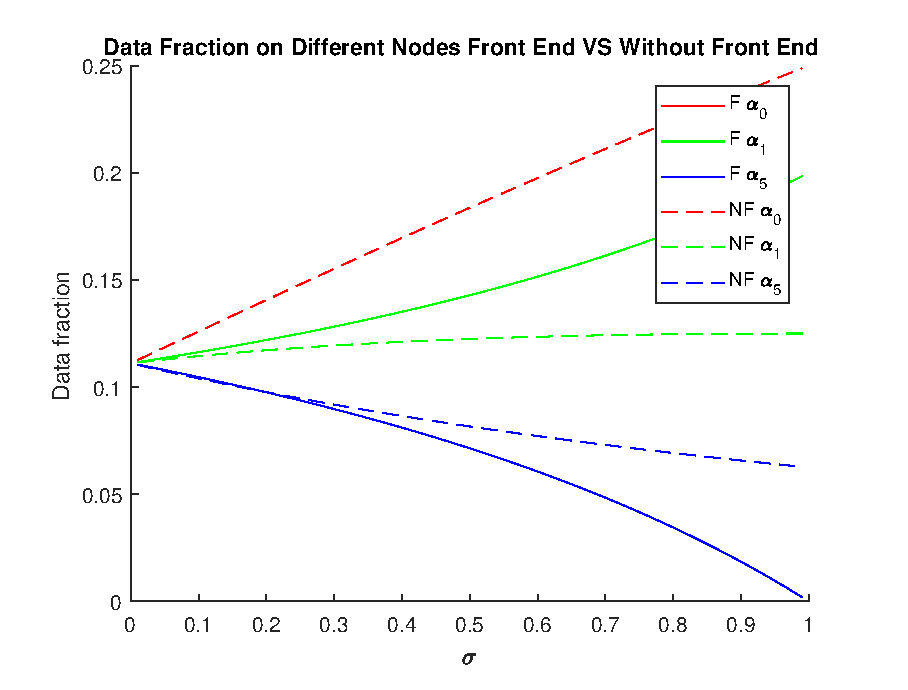
\includegraphics[width=1\columnwidth]{figure/3t3i_c.eps}
\caption{The comparing result between front-end processor with without front-end processor in 3*3 regular network injection on inner grid processor }
\label{fig:3t3i_c}
\end{figure}

\Fig{3t3i_c} says that $P_{0}$ takes more assigned task in without front-end scenario than front-end processor situation.  As the $\sigma$ value goes up, the fractions are deployed to the deeper levels dropping down.  In the limit condition, for example, $\sigma  = 1$,  there is no data transmitted to $level_{2}$, that is, $P_{5}$, $P_{6}$, $P_{7}$ and $P_{8}$ in the front-end assumption.  Yet in the without front-end situation,  there is still about $5\%$ data fraction is communicated to $P_{5}$, $P_{6}$, $P_{7}$ and $P_{8}$.  

Comparing with \Fig{3t3b_c}, $P_{0}$ takes less workload in inner grid position than boundary data injection.  The reason is there are 4 neighbor processors on the $level_{1}$, yet there is solely three processors on $level_{1}$ on the boundary.
\newpage 

\begin{figure}[!ht]
\centering
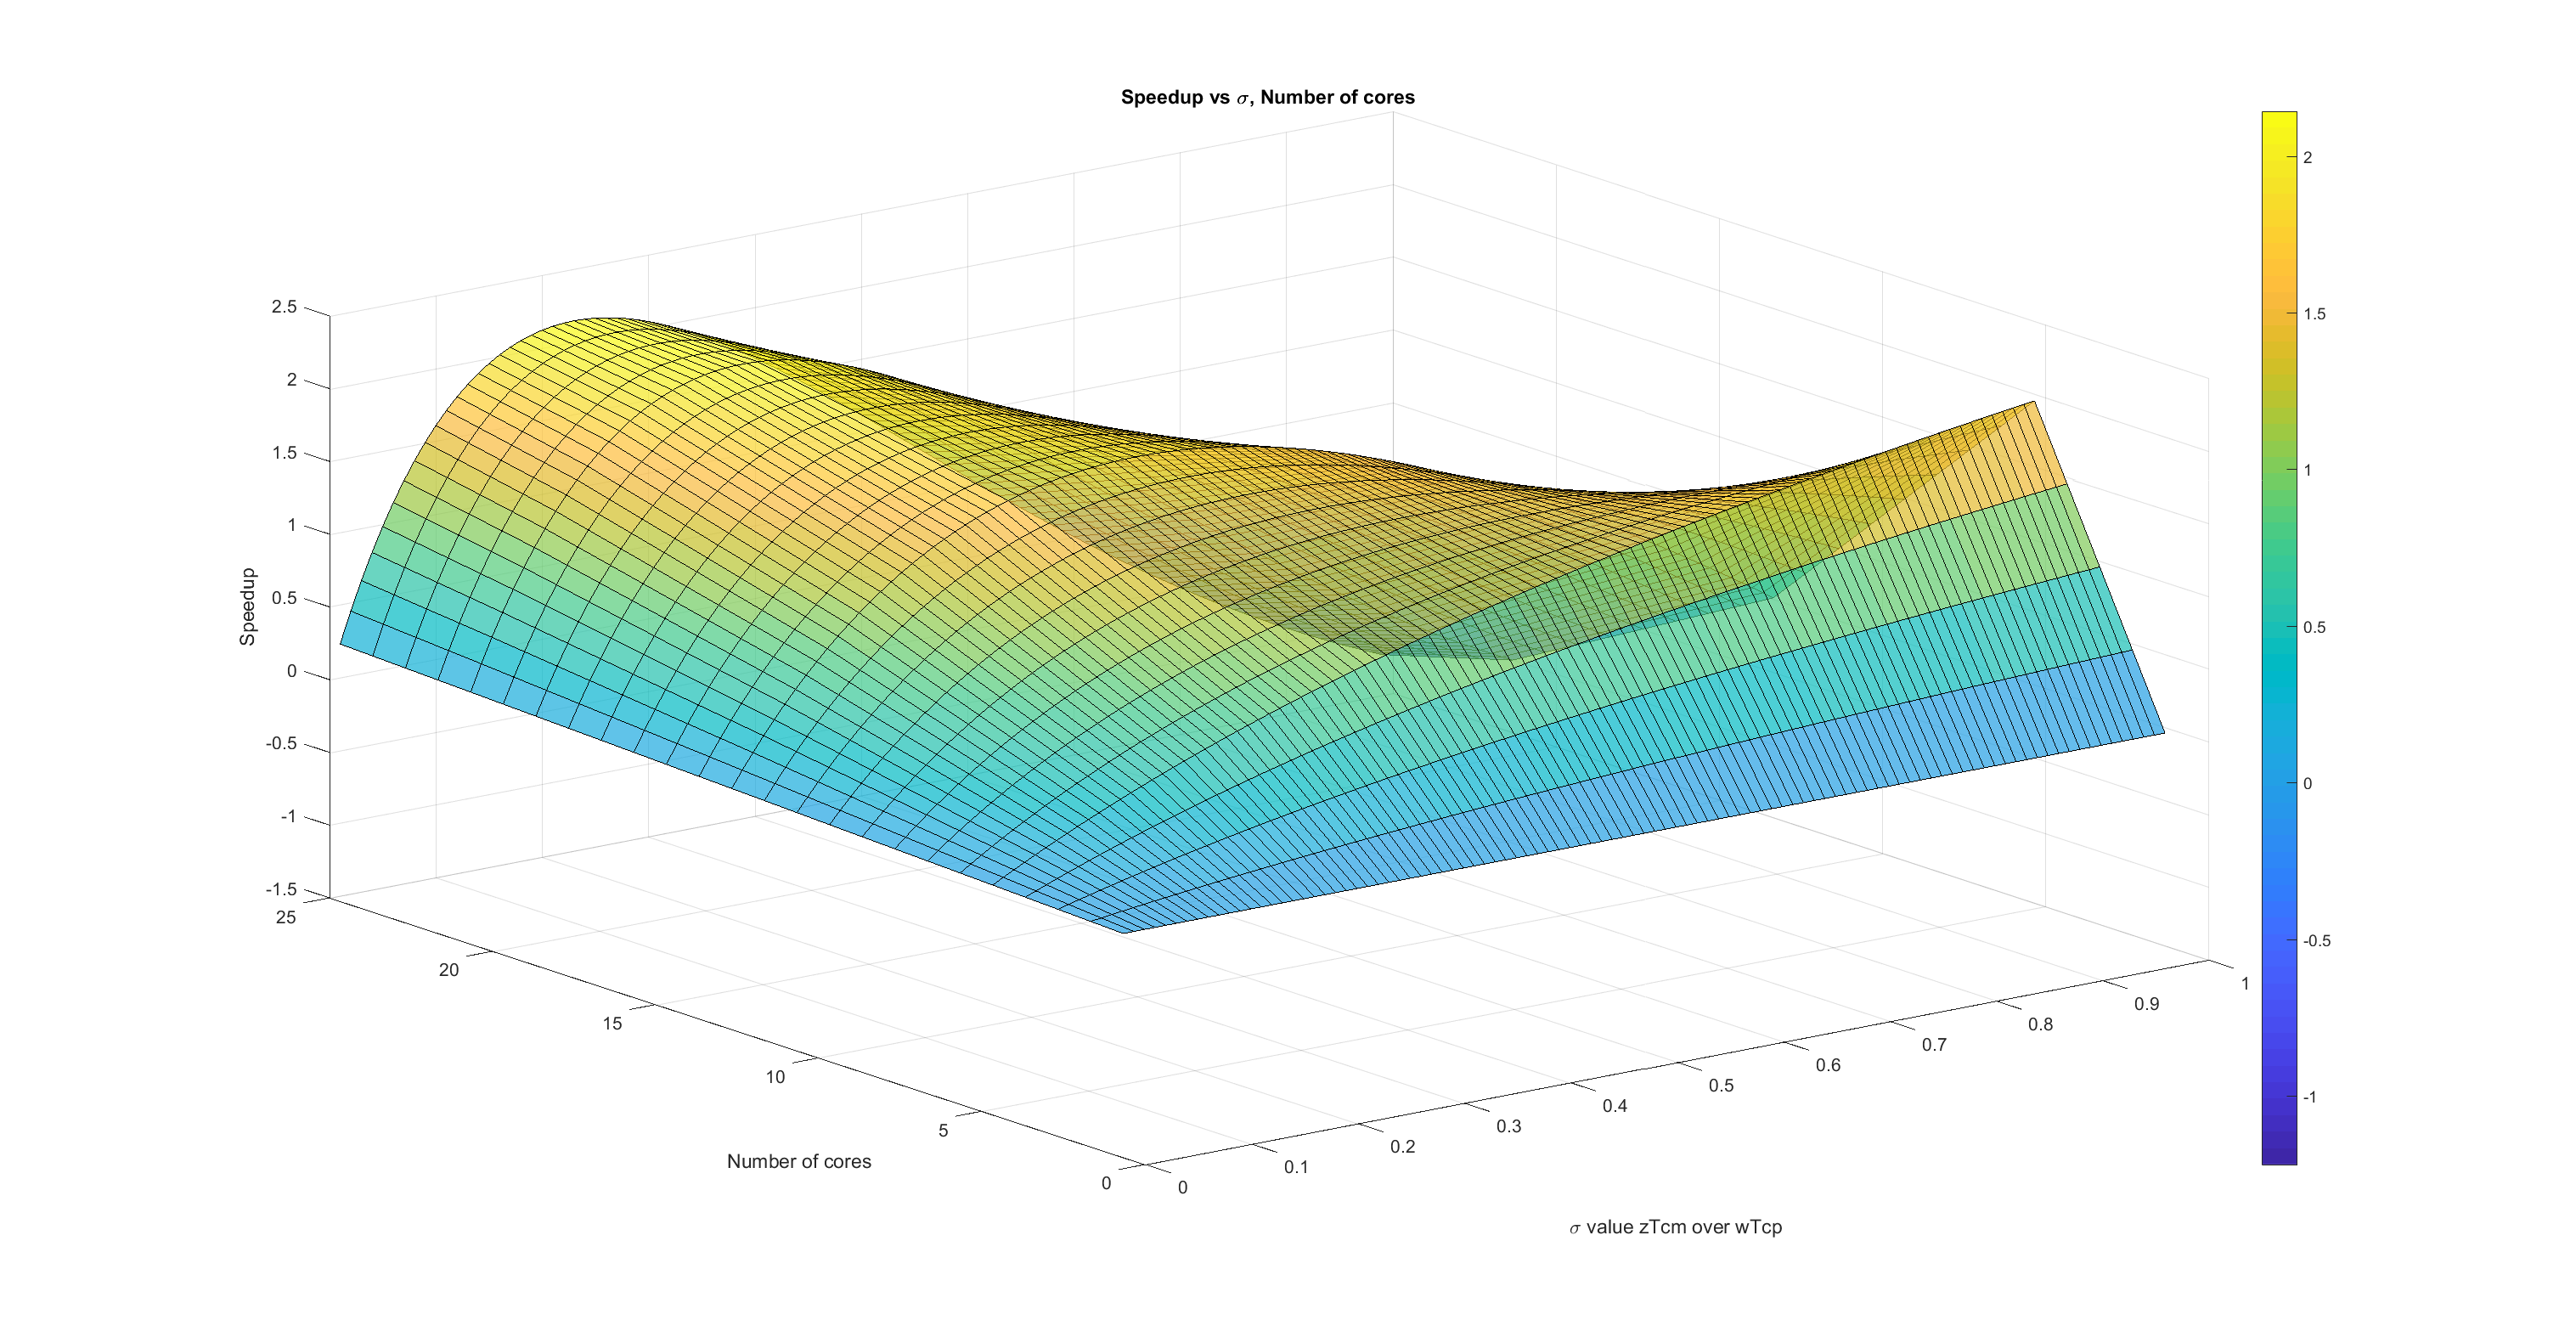
\includegraphics[width=1\columnwidth]{figure/sacom5t5f_nof.eps}
\caption{ Speedup difference between front-end and without front-end in 5*5 regular network}
\label{fig:sacom5t5f_nof}
\end{figure}

\Fig{sacom5t5f_nof} shows the speedup difference between the front-end situation and without front-end scenario.  


\newpage
\section{Store and Froward Switching}
In this chapter, we mainly discuss the virtual cut through \cite{kermani1979virtual} switching.  In addition, the store and froward \cite{kanthraj2007store} schema is a mature data processing technique.  In future works, we discuss it.
